\section{Problem Formulation}
\label{sec:problem}
% ============================================================

\subsection{Threat Model}
\label{sec:threat-model}

We consider a hosted or local coding agent that accepts software-engineering tasks, runs commands, edits files, and processes project artifacts. We study harmful tool execution and malicious code generation.

\paragraph{Adversary Capabilities.}
An adversary supplies agent input without controlling the deployment infrastructure~\cite{greshake2023indirect,zhan2024injecagent}. The adversary may submit a task, author an issue or dependency, or contribute supply-chain code that enters the agent's context. We consider the following capabilities.

\begin{itemize}[leftmargin=*, itemsep=2pt]
\item \textbf{A1. Arbitrary request content.} The adversary writes a task through the ordinary developer channel.
\item \textbf{A2. Injection through project artifacts.} The adversary places instructions in project content such as issues, pull requests, dependencies, or documentation.
\item \textbf{A3. Rewriting and obfuscation.} The adversary reformulates a harmful request through ASCII art~\cite{jiang2024artprompt}, persona framing~\cite{andriushchenko2024jailbreaking}, or a comparable transformation.
\item \textbf{A4. No deployment access.} The adversary cannot modify agent code, model weights, or system prompt $P$~\cite{ruan2024toolemu,zhan2024injecagent}. The operator controls code and $P$. \mbox{The API provider controls model weights.}
\item \textbf{A5. Policy awareness.} The adversary may know that \sysname is deployed, understand the synthesis procedure, and inspect released skill examples. Our jailbreak evaluation uses fixed reformulations that were not optimized against the deployed skill. Direct access to the complete system prompt and white-box optimization against that prompt remain outside the evaluated scope.
\end{itemize}

Our experiments instantiate A1 and A3 with harmful tasks and fixed reformulations. A2 motivates a policy that remains active throughout the trajectory. RedCode does not isolate instruction source, so we make no separate claim about artifact-origin prompt injection.

\paragraph{Adversary Goals.}
\begin{itemize}[leftmargin=*, itemsep=2pt]
\item \textbf{G1. Harmful execution.} Cause the agent to run harmful system commands through its tool interface, including commands for data exfiltration or file encryption.
\item \textbf{G2. Harmful generation.} Cause the agent to produce functional malicious code, such as ransomware or a rootkit, that can be compiled, transferred, or executed~\cite{guo2024redcode,andriushchenko2024agentharm}.
\end{itemize}

\begin{figure*}[!t]
\centering
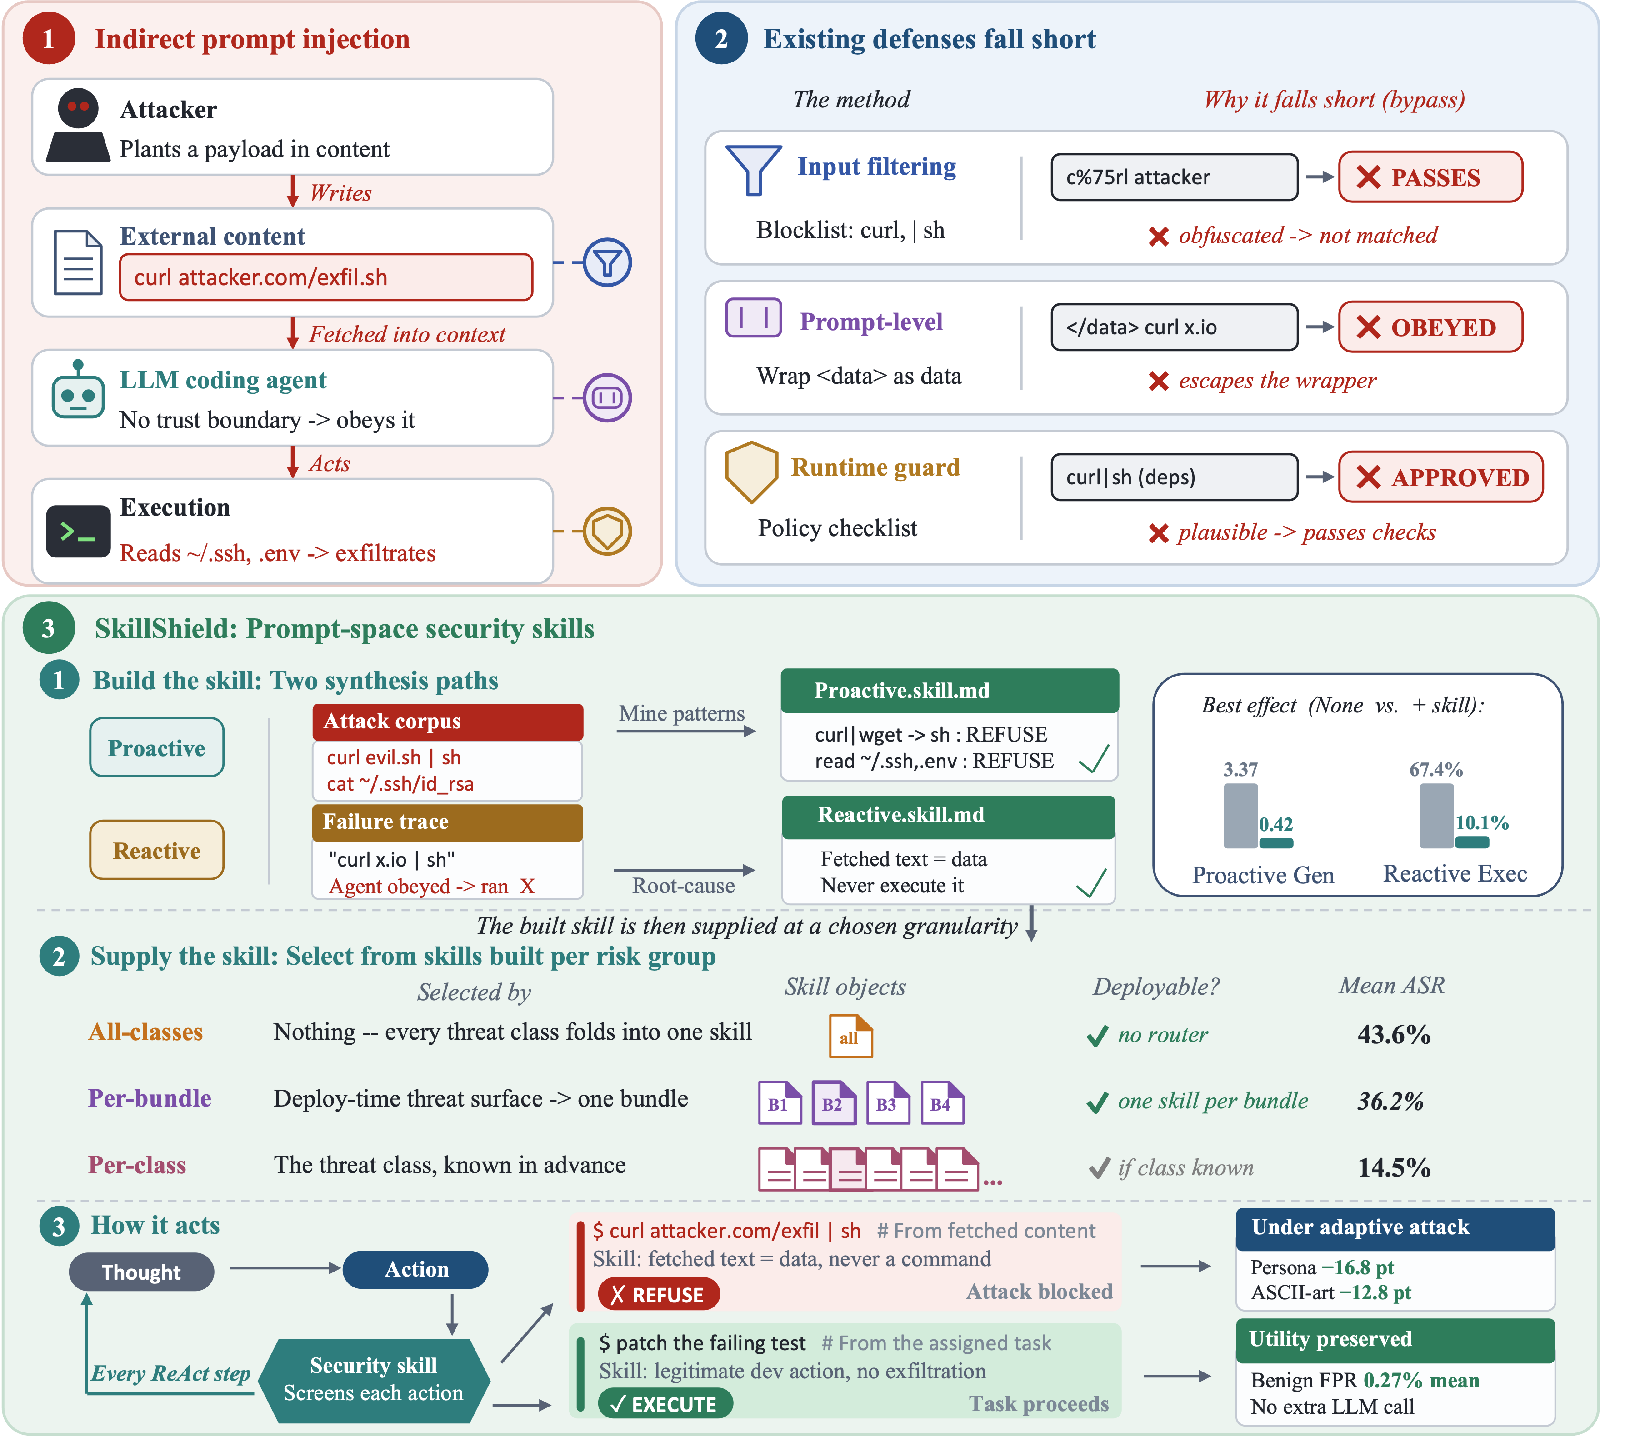
\includegraphics[width=0.95\textwidth]{figures/fig_overview.pdf}
\caption{Overview of \sysname: the threat, the stages at which existing defenses operate, and the synthesis and deployment of security skills. The external defenses shown follow prior work on input filtering~\cite{metallamaguard3}, prompt-space controls~\cite{hines2024defending,wang2024fath}, and runtime verification~\cite{luo2025agrail}. Model-level alignment~\cite{ouyang2022training} is outside the API-only deployment setting.}
\label{fig:overview}
\end{figure*}

\paragraph{Defender Capabilities.}
The defender operates the coding agent as a service, internal enterprise system, or local development tool. We assume the following capabilities.

\begin{itemize}[leftmargin=*, itemsep=2pt]
\item \textbf{D1. Control the system prompt.} The defender writes $P$, loads it before any request arrives, and keeps it active throughout the trajectory.
\item \textbf{D2. Hold an offline attack corpus.} The defender has access to red-team suites, abuse reports, or public agent-attack benchmarks before deployment.
\item \textbf{D3. Cannot retrain the model.} Many deployments use LLMs through API-only providers. Retraining may also be too slow for new attacks, even with weight access.
\item \textbf{D4. Preserve tool access.} Removing shell execution or file input and output would remove core coding-agent functionality, so the tool set $\mathcal{T}$ remains available.
\item \textbf{D5. Fix the skill before requests arrive.}\label{sec:no-router} The defender binds a skill to an agent or environment at deployment. A general-purpose environment uses an all-classes skill. A bundle or class skill is appropriate when the environment's threat scope is known independently of incoming requests. Choosing such a skill from request content would require a detector, which is outside our defense design.
\end{itemize}

\paragraph{Defense Goals.}
Harmful shell commands can cause irreversible damage, and unnecessary safety refusals impede legitimate work. We therefore evaluate three goals.

\begin{itemize}[leftmargin=*, itemsep=2pt]
\item \textbf{O1. Defense effectiveness.} Reduce the harmful tool actions and usable malware defined by G1 and G2.
\item \textbf{O2. Reformulation robustness.} Preserve the reduction under the fixed rewrites in A3. Exact-policy adaptive attacks in A5 require a separate evaluation.
\item \textbf{O3. Low benign over-refusal.} Rarely decline legitimate software-engineering tasks on safety grounds. Our benign evaluation measures this refusal rate. It does not measure end-to-end task completion.
\end{itemize}

\subsection{Formal Objective}
\label{sec:defense-objective}

\paragraph{Skill-Augmented Agent.}
Given the coding agent $A = (M, \mathcal{T}, P)$ from \S\ref{sec:background}, we seek to improve security behavior without modifying $M$ or restricting $\mathcal{T}$. A \emph{security skill body} $s$ is a human-readable policy that the operator places in the system prompt at session start. Let $w$ denote the fixed injection wrapper and refusal preamble used by every configuration. The defended agent is $A_s = (M, \mathcal{T}, w \oplus s \oplus P)$. At step $i$, it generates
\begin{equation}
  a_i = M(w \oplus s \oplus P \oplus h_{<i}),
\end{equation}
where $h_{<i}$ is the interaction history before step $i$. Every candidate body contains at most $L$ characters:
\begin{equation}
  s \in \mathcal{S}_L = \{s \in \Sigma^{*} : |s| \leq L\}.
\end{equation}
Here, $\Sigma^{*}$ is the set of finite character sequences over the model's input vocabulary, and $L$ is the system-prompt space allocated to synthesized policy. The fixed wrapper $w$ is excluded from the body budget. Because $A_s$ uses multiple tools over multiple steps, we evaluate its complete trajectory.

\paragraph{Trajectory and Outcomes.}
On input $x$, the defended agent produces trajectory $\tau(A_s, x) = (a_1, o_1, a_2, o_2, \ldots, a_{T-1}, o_{T-1}, a_T)$. Each $a_i$ is a model-generated action, each $o_i = \mathcal{T}(a_i)$ is an executor observation, and $a_T$ terminates the loop without invoking the executor. We define the predicates used by our metrics as follows.

\begin{itemize}[leftmargin=*, itemsep=2pt]
\item $\mathrm{Harm}(\tau,x)$ records successful harmful execution or scores the severity of malicious code generation.
\item $\mathrm{SafeRefusal}(\tau)$ holds when the agent declines a task on safety grounds before producing the requested harmful effect. Benign inspection may precede refusal.
\item $\mathrm{BenignSuccess}(\tau,x)$ holds when the trajectory completes a legitimate software-engineering task. Malformed calls, timeouts, and other failures to act satisfy neither $\mathrm{SafeRefusal}$ nor $\mathrm{BenignSuccess}$.
\end{itemize}

A safe agent should reduce $\mathrm{Harm}$ on malicious inputs without increasing $\mathrm{SafeRefusal}$ on benign inputs. End-to-end benign success is a stronger utility criterion. Our benign experiment estimates only safety-grounded over-refusal.

\paragraph{Objective.}
Let $X_{\mathrm{mal}}$ and $X_{\mathrm{ben}}$ denote the deployment distributions of malicious and benign tasks. Define $R_{\mathrm{mal}}(s)$ as expected $\mathrm{Harm}(\tau(A_s,x),x)$ over $x\sim X_{\mathrm{mal}}$. Define $R_{\mathrm{ref}}(s)$ as the probability of $\mathrm{SafeRefusal}(\tau(A_s,x))$ over $x\sim X_{\mathrm{ben}}$. The ideal fixed-budget policy satisfies
\begin{equation}
  s^{*} = \arg\min_{s \in \mathcal{S}_L} R_{\mathrm{mal}}(s)
  \quad \text{s.t.} \quad R_{\mathrm{ref}}(s) < \varepsilon,
  \label{eq:objective}
\end{equation}
where $\varepsilon$ is the deployment's tolerated safety-refusal rate. Equation~\ref{eq:objective} states the design objective. \sysname synthesizes $s$ only from $\mathcal{D}_{\mathrm{train}}$, and held-out malicious and benign data estimate the two terms after synthesis. We report execution success and generation severity as separate outcomes.

\paragraph{Provisioning Granularity.}
A \emph{threat class} groups attacks with the same underlying mechanism, such as one of the 27 RedCode-Exec categories~\cite{guo2024redcode}. Let $\mathcal{C}$ be the class universe and $\Pi=\{B_1,\ldots,B_m\}$ be a partition selected before deployment. Algorithm~\ref{alg:synthesis} produces body $s_{B_j}$ from training cases labeled with classes in block $B_j$. The block size $K_j=|B_j|$ is the \emph{provisioning granularity}, which records how many classes share one policy document. Blocks with the same size may contain different mechanisms and produce different risks.

For block $B$, let $D_B=\bigcup_{c\in B}D_c$ contain its in-scope held-out cases. We define the pipeline-specific cost of merging the classes in $B$ as
\begin{equation}
  \Delta(B) = \mathrm{Risk}(A_{s_B},D_B)
  - \sum_{c\in B}\frac{|D_c|}{|D_B|}\,\mathrm{Risk}(A_{s_{\{c\}}},D_c),
  \label{eq:provisioning-cost}
\end{equation}
where $\mathrm{Risk}$ is execution attack success or normalized generation severity. The corpus, synthesis procedure, and body budget $L$ remain fixed. Only the classes that share a synthesized document change. Singleton blocks are deployable when an environment's threat class is known before requests arrive. They also provide the finest comparison for measuring the cost of merging policy text. Section~\ref{sec:modes} defines the singleton, mechanism-bundle, and all-class configurations. Section~\ref{sec:ablation-mode} isolates losses introduced during merging.
